% Section content template for individual Educative lessons
% This file contains the actual content for a specific section
% Generated from Educative API section content

% Section: System Design: A Blob Store
% Section ID: 4862646238576640
% Section Slug: system-design-a-blob-store
% Generated: 2025-12-07T21:36:17.715782

\subsection{What is a blob store?}\label{0t_3XqY5eDWyO-7KGPQxc}
\\
\textbf{Blob store} is a storage solution for unstructured data.
\\
We can store photos, audio, videos, binary executable codes, or other multimedia items in a blob store. Every type of data is stored as a blob(A blob (binary large object) consists of a collection of binary data stored as a single unit.). It follows a flat data organization pattern, where there are no hierarchies, such as directories and subdirectories.
\\
Mostly, it's used by applications with a specific business requirement called~\textbf{write once, read many (WORM)}, which states that data can only be written once and cannot be changed.
\\
Just like in Microsoft Azure, the blobs are created once and read many times. Additionally , these blobs can't be deleted until a specified interval, and they also can't be modified to protect critical data.

\begin{figure}[htbp]
 \centering
 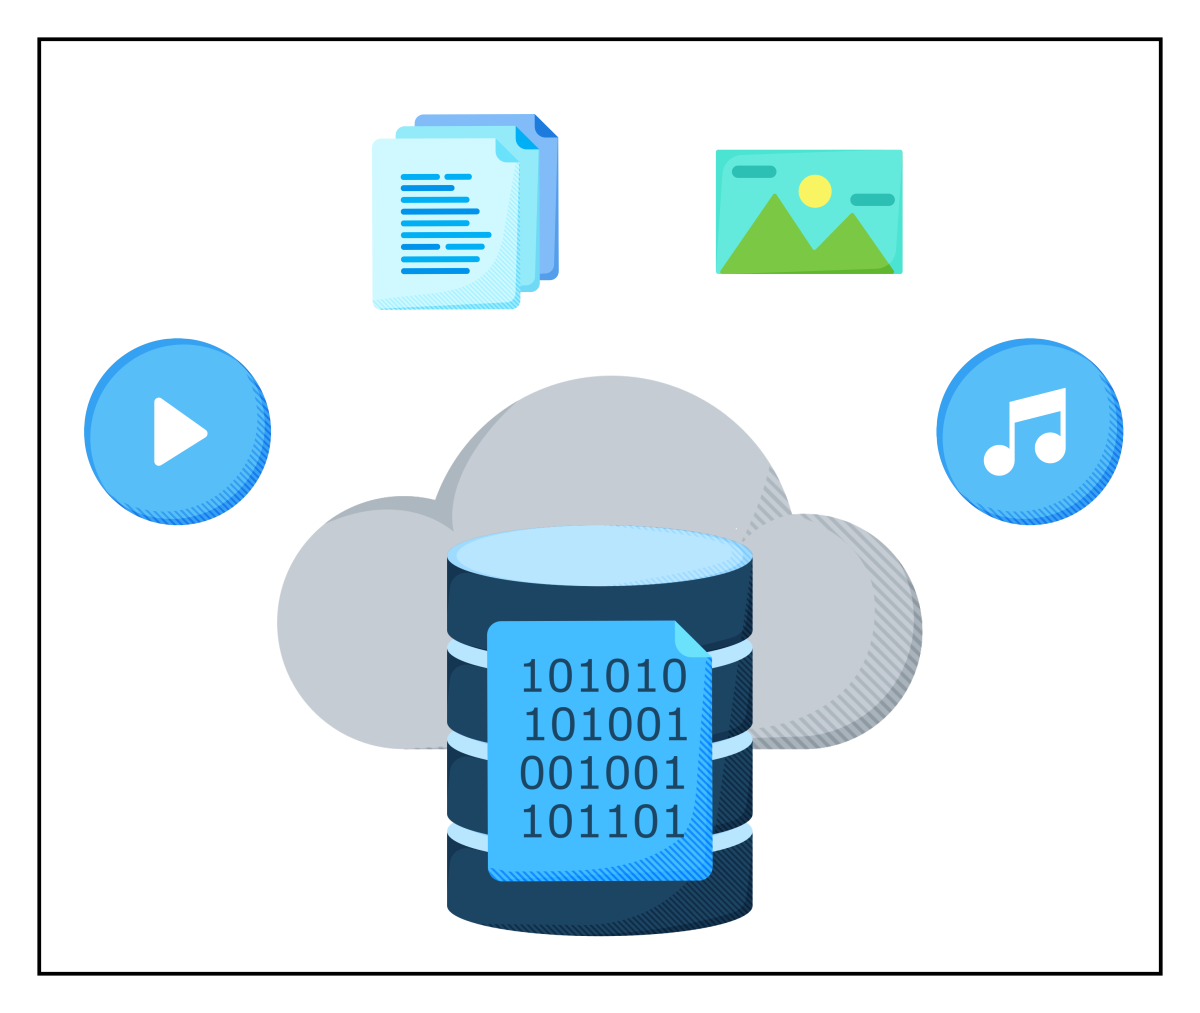
\includegraphics[width=0.25\textwidth]{Images/chapter_20/section_4862646238576640/6638802153897984.png}
 \caption{A blob store storing and streaming large unstructured files like audio, video, images, and documents}
\end{figure}

\textbf{Note:} It isn't necessary for all applications to have this WORM requirement. However, we assume that the blobs written can't be modified. Instead of modifying, we can upload a new version of a blob if needed.

\subsection{Why do we use a blob store?}\label{why-do-we-use-a-blob-store}
\\
Blob store is a crucial component of many data-intensive applications, including YouTube, Netflix, and Facebook.
\\
The table below shows the blob storage used by some of the most well-known platforms. These applications generate large volumes of unstructured data daily and require a storage solution that is scalable, reliable, and highly available, particularly for storing large media files.
\\
As their data continues to grow, these applications also need the ability to store an unlimited number of blobs.
\\
According to some estimates, YouTube adds more than a petabyte of new storage each day. In a system like YouTube, each video is stored in multiple resolutions, and every resolution is replicated across multiple data centers and regions to ensure redundancy and availability.
\\
This is why the total storage required for each video is significantly higher than the original upload size.

\begin{table}[htbp]
\centering
\small
\adjustbox{max width=\textwidth}{
\begin{tabular}{|p{0.475\textwidth}|p{0.475\textwidth}|}
\hline
\textbf{System} & \textbf{Blob Store} \\
\hline
\hline
Netflix & S3 \\
\hline
YouTube & Google Cloud Storage \\
\hline
Facebook & Tectonic \\
\hline
\end{tabular}
}
\end{table}

With the importance of blob storage established, the next step is to understand how cloud providers, such as Azure, optimize costs and performance through different storage access tiers.

\subsection{Azure storage access tiers}\label{rdv4DttQETC0pGQZ_NyFm}
\\
Azure storage access tiers offer cost-effective storage options tailored to the various usage patterns and access frequencies of our data.

\begin{figure}[htbp]
 \centering
 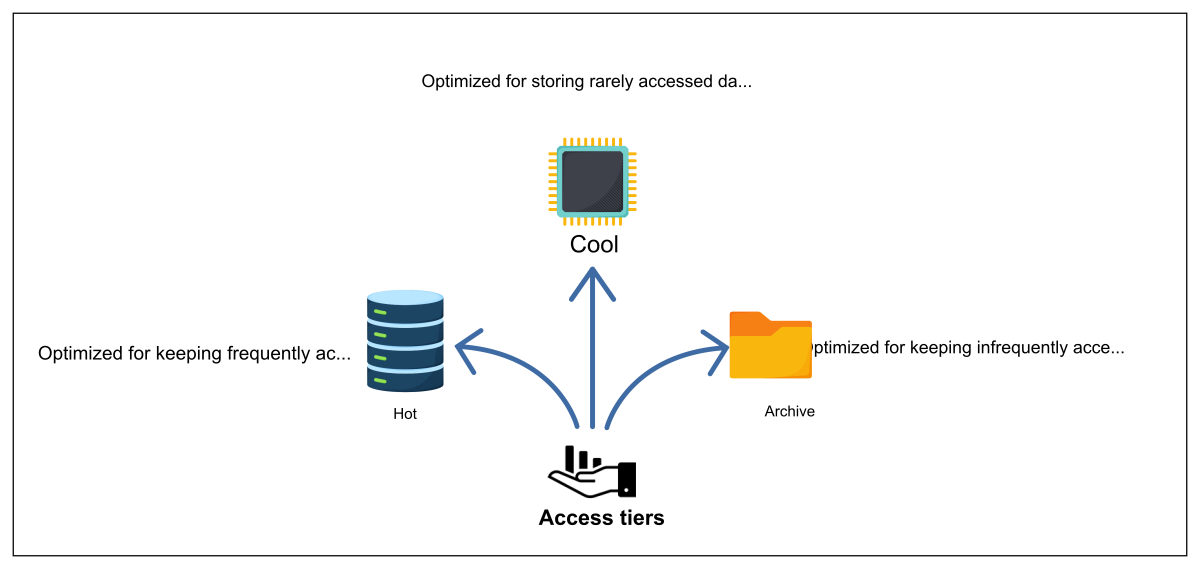
\includegraphics[width=0.5\textwidth]{Images/chapter_20/section_4862646238576640/5495555775922176.png}
 \caption{Azure Storage access tiers }
\end{figure}

\begin{quote}
\textbf{Note:}~We can change between these access tiers at any moment.
\end{quote}

\begin{center}
{\def\LTcaptype{none} % do not increment counter
\begin{longtable}[]{@{}
>{\raggedright\arraybackslash} p{(\linewidth - 4\tabcolsep) * \real{0.3333}}
>{\raggedright\arraybackslash} p{(\linewidth - 4\tabcolsep) * \real{0.3333}}
>{\raggedright\arraybackslash} p{(\linewidth - 4\tabcolsep) * \real{0.3333}}@{}}
\toprule\noalign{}
\endhead
\bottomrule\noalign{}
\endlastfoot
\begin{minipage}[t]{\linewidth}\raggedright
\textbf{Feature}
\end{minipage} & \begin{minipage}[t]{\linewidth}\raggedright
\textbf{Description}
\end{minipage} & \begin{minipage}[t]{\linewidth}\raggedright
\textbf{When to Use}
\end{minipage} \\
\begin{minipage}[t]{\linewidth}\raggedright
\textbf{Azure files}
\end{minipage} & \begin{minipage}[t]{\linewidth}\raggedright
\begin{itemize}
\item
Provides a Server Message Block (SMB) interface
\item
Provides client libraries
\item
Includes a REST interface for remote file storage
\end{itemize}
\end{minipage} & \begin{minipage}[t]{\linewidth}\raggedright
\begin{itemize}
\item
Cloud application migration (lift and shift)
\item
Data sharing across several virtual machines
\item
Keeping development and debugging tools available on many virtual computers
\end{itemize}
\end{minipage} \\
\begin{minipage}[t]{\linewidth}\raggedright
\textbf{Azure blobs}
\end{minipage} & \begin{minipage}[t]{\linewidth}\raggedright
\begin{itemize}
\item
Provides client libraries
\item
Provides a REST interface for massively storing and retrieving unstructured data in block blobs
\end{itemize}
\end{minipage} & \begin{minipage}[t]{\linewidth}\raggedright
\begin{itemize}
\item
Remote access to application data
\item
Support for streaming and random-access scenarios
\end{itemize}
\end{minipage} \\
\end{longtable}
}
\end{center}

Let's examine the blob lifecycle management rules for effective data management solutions in Azure blob storage.

\subsection{Blob life cycle management rules}\label{bFcikMju76m-r_nKWpVDv}
\\
Blob life cycle management rules simplify data management in Azure Blob Storage, improving cost efficiency, data retention compliance, and overall organization, while ensuring effective and seamless data life cycle management.
\\
Here are the blob life cycle management rules:

\begin{itemize}
\item
\protect\phantomsection\label{XoHaQvOr_maHyq91j8WJo}
\textbf{Moving blobs to a cooler storage layer can improve performance and save costs:} Blob life cycle management rules enable us to transfer data from a hot access tier to a cool access tier when it is accessed less frequently, resulting in cost savings without affecting accessibility.
\item
\protect\phantomsection\label{j3zvw-vueDl8hr3NeI3CX}
\textbf{Deleting blobs at the end of their life cycle:}~We may use these rules to create criteria, such as expiry dates or inactivity levels, to automatically destroy outdated or obsolete blobs, thereby facilitating data management and ensuring compliance.
\item
\protect\phantomsection\label{OHqppa4jKzG86kPyIXQzt}
\textbf{Applying rules to filtered paths in the Storage account:}~We can selectively apply life cycle rules to specific folders or containers within our Storage account, tailoring the automated actions to our data organization and access patterns.
\end{itemize}
\\
To see these concepts in action, let's examine common real-world scenarios where blob storage plays a critical role.

\subsection{Use cases}\label{GWfuHH4lhkabt7-r0FlLg}
\\
Blob storage is highly versatile and powers many real-world applications that require the efficient storage, access, or delivery of large amounts of unstructured data. Here are some common scenarios:

\begin{itemize}
\item
\protect\phantomsection\label{PHfb-4lgqCWM1EN3BG9pP}
Serving pictures or documents to browsers immediately.
\item
\protect\phantomsection\label{IfOIo_Xw97UXs3pkcmySa}
Storing documents for multiple users.
\item
\protect\phantomsection\label{E2B_jbCJxgRabrW_rd2cn}
Broadcasting audio and video content.
\item
\protect\phantomsection\label{1qSzvVshMkEAHhQuCGa2r}
Maintaining data for backup and restore, recovery from disasters, and archiving.
\item
\protect\phantomsection\label{7gw3fF4cs9snWSbu9PQBB}
Data storage for analysis via an on-premises or Azure-hosted service.
\end{itemize}
\\
These examples demonstrate how blob storage provides a reliable, scalable, and cost-effective solution for a wide range of applications, from media streaming to enterprise data management. With the principles, tiers, and life cycle management in mind, we are now ready to translate these concepts into a practical, step-by-step blob store System Design.

\subsection{How do we design a blob store system?}\label{wI8Z8ozI8EVzgZO9o6x2o}
\\
We have divided the design of the blob store into five lessons and a quiz.

\begin{enumerate}
\item
\protect\phantomsection\label{64X0SL-QgKdiY8htgzLAj}
\href{https://www.educative.io/courses/grokking-the-system-design-interview/requirements-of-a-blob-stores-design}{\textbf{Requirements:}} In this lesson, we identify the functional and non-functional requirements of a blob store. We also estimate the resources required by our blob store system.
\item
\protect\phantomsection\label{sCSftNcTBUbXsyOltwr3x}
\href{https://www.educative.io/courses/grokking-the-system-design-interview/design-of-a-blob-store}{\textbf{Design:}} This lesson presents a high-level design, the API design, and a detailed design of the blob store, while explaining the details of all components and the workflow.
\item
\protect\phantomsection\label{MhchOsnFOHROFzPE9VuOT}
\href{https://www.educative.io/courses/grokking-the-system-design-interview/design-considerations-of-a-blob-store}{\textbf{Design}} \href{https://www.educative.io/courses/grokking-the-system-design-interview/design-considerations-of-a-blob-store}{\textbf{Considerations:}}~In this lesson, we discuss several key aspects of design. For example, we learn about the database schema, partitioning strategy, blob indexing, pagination, and replication.
\item
\protect\phantomsection\label{XY0fxBfzE2C17dv8ZtO-y}
\href{https://www.educative.io/courses/grokking-the-system-design-interview/evaluation-of-a-blob-stores-design}{\textbf{Evaluation:}} In this lesson, we evaluate our blob store based on our requirements.
\item
\protect\phantomsection\label{bS37V2LcUsnGZU0uJP7we}
\href{https://www.educative.io/courses/grokking-the-system-design-interview/quiz-on-the-blob-stores-design}{\textbf{Quiz:}} In this lesson, we assess understanding of the blob store design.
\end{enumerate}
\\
Let's start with the requirements of a blob store system.

% End of section content